\chapter{Aplicación del método}
\label{Metodo}
El desarrollo de la metodología propuesta en el proyecto es el capítulo central de este documento, aquí se presenta el diseño y la implementación de los algoritmos desarrollados en el proyecto.


%En seguida, se inicia con la presentación de trabajos que dejan ver la importancia que este tipo de propuestas tiene para la comunidad científica internacional.


%\section{DISEÑO DEL PROTOTIPO} 
%Aquí se describe cada uno de los componentes del diseño que compone esta investigación.

\section{Diseño del grafo}
\textit{Inspirados en el grafo del caso de estudio descrito en la sección \ref{Sec:CMMN}, se observó que en la notación de modelado CMMN (ver figura \ref{EjCMMN}) se cuenta con un conjunto de tareas o actividades y de flujos entre ellas, que pueden ser opcionales. Se vio cómo esta situación podía modelarse en un grafo, en el que el problema a solucionar consiste en qué tareas realizar de \textbf{L} etapas consecutivas, para alcanzar al final el objetivo.}

\textit{Un grafo dirigido y conexo permite modelar la estructura de procesos de decisión por etapas de estado y tiempo finitos, como el se aprecia en la figura \ref{GrafoEtapas}, cuyos nodos, entre cada dos etapas, tienen las características de un grafo bipartito, es decir que, entre acciones de la misma etapa no deben existir aristas; además, como es conexo, se garantiza que exista al menos una arista que conecte dos etapas sucesivas, así, cada nodo, (excepto los de la última etapa), debe estar conectado al menos con un nodo de la etapa siguiente. }

\begin{figure}[H]
  \centering
    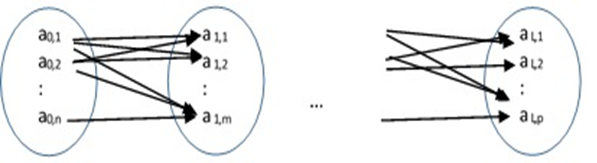
\includegraphics[scale=0.8]{GrafoEtapas.png}
  \caption{Grafo con L etapas}
  \label{GrafoEtapas}
\end{figure}

\textit{El grafo es un <<grafo por etapas>>, característica definida en la sección \ref{ConcepGraph}, y el problema que se quiera modelar debe asemejarse a este grafo de $L$ etapas, para que sea susceptible de emplear la aplicación propuesta en esta tesis con la cual encontraría un camino recomendable para alcanzar un objetivo dado.}

\section{Diseño del modelo matemático}
\label{mat}
La fórmula \ref{for:2}, como sucede con la distribución de \textit{SoftMax}, permite normalizar las probabilidades para que correspondan a cantidades positivas menores o iguales a 1, pero con un fácil cálculo de la sudatoria del denominador, dados los valores de A que corresponden a ceros o a unos. 

\begin{eqnarray}\label{for:2}
P(i \to j) = \frac{e^{v_j}}{\sum_k A_{i,k} e^{v_k}},
\end{eqnarray}


Así, la cantidad del numerador siempre será inferior o,  a lo sumo, igual a la cantidad del denominador, dado que el numerador es parte de la sumatoria del denominador, que, adicionalmente, es de valores positivos. La multiplicación por el valor de cada posición en la matriz de adyacencia $A$, garantiza que únicamente se sumen los exponenciales de nodos a los que en realidad se accede. 

Otra característica de esta fórmula es que con los valores iniciales en cero para los exponentes de $e$, se obtienen probabilidades uniformes para todo nodo $j$ adyacente al nodo $i$.

Finalmente, para controlar el aprendizaje del autómata se incrementa o decrementa el valor del exponente de la fórmula anterior, dado que de esta forma aumenta o disminuye la probabilidad asociada al nodo relacionado. Esto puede verse en la fórmula sencilla \ref{for:3}.
\begin{eqnarray}\label{for:3}
v_j(\tau + 1) = v_j(\tau) + \delta,
\end{eqnarray}

donde $\delta$ es un parámetro que controla la rata de aprendizaje:

$P(i \to j)_{\tau+1} \sim e^{\delta} P(i \to j)_{\tau}$ 

para pequeños valores de $\delta$.



Cada uno de los nodos del grafo se constituye en un \textit{ bandit}, pero la recompensa de pasar por cada uno de ellos se desconoce antes y después de ello y solo se conocerá al finalizar la secuencia total de acciones que se decida tomar, es decir, al final de las \textbf{L} etapas.

Como la probabilidad total de una ruta determinada, equivale a multiplicar las probabilidades de ir de un nodo a otro hasta culminar la ruta, tal como se hace en un árbol Bayesiano y como se presenta en la fórmula \ref{model1}, al tener el valor de recompensa de haber seleccionado un camino, se decide afectar las probabilidades de pasar entre cada uno de sus nodos, lo que se reflejará en una matriz de probabilidades de transición de estados, donde los estados son los nodos del grafo.
\begin{eqnarray}\label{model1}
P(i_{0} \to i_{1}, ... i_{l-1} \to i_{l}, ... i_{L-1} \to i_{L})=P(i_{0} \to i_{1})P(i_{1} \to i_{2})...P(i_{L-1} \to i_{L}),
\end{eqnarray}
donde $i$ denota el nodo seleccionado en cada una de las etapas, su subíndice $l=0,1,...,L$ denota la etapa a la que pertenece y L denota el número total de etapas. 

Cuando $l = L$ se habrá acumulado una ganancia $G$, que puede ser positiva o negativa. Dado este valor, se hace una modificación a cada una de las probabilidades de transición involucradas y se constituye en el modelo de aprendizaje que se explicará en la sección \ref{aprende}.

Estas probabilidades se pueden aproximar mediante la fórmula \ref{model2}, que garantiza la normalización de las probabilidades de transición desde un mismo nodo, cuya suma se requiere que sea 1.
\begin{eqnarray}\label{model2}
P(i \to j) = \frac{e^{v_j}}{\sum_k A_{i,k} e^{v_k}},
\end{eqnarray}
donde $A$ es la matriz de adyacencia del grafo y, el valor binario de $A_{i,k}$ permite que solo se tengan en cuenta nodos alcanzables desde el nodo $i$; además, $v$ es el valor asociado a cada uno de los nodos del grafo, el cual se va actualizando en cada una de las iteraciones $\tau$ como se muestra en la ecuación \ref{model3}, valor que no necesariamente está relacionado con la recompensa asociada a ese nodo (\textit{bandit}).

Los valores iniciales de los $v$ son cero, de forma que la fórmula \ref{model2} calcula la misma probabilidad para pasar de un nodo a cada uno de sus siguientes o vecinos alcanzables, es decir, con una probabilidad uniforme, garantizando que la decisión inicial de pasar del nodo $i$ a otro nodo $k$, es totalmente aleatoria.

\textit{La probailidad de transición del estado i al estado j es proporcional al valor de utilidad que da esa decisión. Mediante la fórmula se quiere orientar a lagente para que sepa en cada etapa y en cada nodo de una etapa la transición más recomendable que a la larga va a dar el mayor beneficio}

\textit{Es una particularización de un problema muy general de Aprendizaje por refuerzo o de problemas de decisión de Markov que se resuelven mediante muestreo de Boltsman (Caso especial: aprovechar la estructura del Grafo por etapas)}

\section{Diseño del modelo de aprendizaje} \label{aprende}
Cada uno de los nodos es un \textit{bandit}; en la etapa uno se selecciona el nodo origen y se estima una ganancia que se genera aleatoriamente a una desviación estándar de su \textit{bandit} y en cada etapa siguiente se selecciona un nodo adyacente al ya seleccionado, inicialmente con una probabilidad uniforme, teniendo en cuenta las restricciones de precedencia del problema. 

La decisión de usar una generación de números aleatorios que siguen una distribución normal con media en cero y desviación estándar en 1, es porque es la utilizada en la literatura de aprendizaje por refuerzo \citep{sutton1992reinforcement}, con la cual se ha probado el funcionamiento del modelo de decisión \textit{n-armed bandit}. 

Posteriormente, aplicando el modelo matemático, se elegirán los nodos de acuerdo con una matriz de probabilidades de transición de estado, que el autómata irá aprendiendo, teniendo en cuenta la fórmula \ref{model2}.

Al culminar la secuencia de nodos de las L etapas, se recibe una recompensa que indicará si se ha alcanzado o no el objetivo. De acuerdo a esta recompensa, la preferencia $v$ de cada nodo de la ruta será ponderada para la siguiente iteración sumando un $\delta$, que puede ser positivo o negativo, como se muestra en la fórmula \ref{model3}
\begin{eqnarray}\label{model3}
v_j(\tau + 1) = v_j(\tau) + \delta,
\end{eqnarray}
donde $\delta$ es un parámetro que controla la rata de aprendizaje: $P(i \to j)_{\tau+1} \sim e^{\delta} P(i \to j)_{\tau}$ para pequeños valores de $\delta$.

%El modelo de decisión es lo suficientemente simple como para admitir un tratamiento bayesiano completo de la estimación de parámetros después de cada episodio. Dada la ganancia total $V_L(\tau) = v_1(\tau)+...+v_L(\tau)$, la probabilidad siguiente $P[\vec{v}(\tau) | V_L(\tau)]$ puede escribirse en términos de la ecuaciones (\ref{model1}) y (\ref{model2}).

Luego de varias iteraciones, la matriz de probabilidades tiende a estabilizarse, es decir, sus valores no cambian considerablemente. De esta forma el modelo ya ha aprendido una ruta específica que reconocerá como la recomendada.

Estos nuevos valores de preferencia de los nodos se tienen en cuenta para calcular una nueva ruta, dando prioridad de selección a los nodos que cuenten con un mayor valor, de acuerdo a la fórmula \ref{model2}, lo que garantiza que, finalmente los nodos con mayor valor de preferencia, quedarán en la ruta solución.

\subsection{Explotación}
La posibilidad de seleccionar con mayor probabilidad los nodos que han estado involucrados en rutas que generan recompensas positivas, permite que el autómata pueda acercarse, cada vez con mayor exactitud, a los valores de los \textit{bandits} que realmente están asociados a cada uno de los nodos de la ruta que él considera que es la más opcionada.

Este aspecto es el que se conoce como explotación que, en términos de juegos de casino, es seguir jugando la misma opción que ha dado los mejores resultados, esperando mejorar aún más.

\subsection{Exploración}
Este modelo de aprendizaje deja la posibilidad de seleccionar en cada etapa un nodo, que no necesariamente sea el que ha venido dando el mejor resultado, porque todos los nodos tendrán alguna posibilidad, aunque sea pequeña, de ser elegidos.

Este aspecto se conoce como la exploración, que consiste en dar un margen de duda, por si hay otras opciones que aún no han sido exploradas y que pueden dar una mejor recompensa.

\section{Selección del camino respuesta}

%\subsection{Modelo Convergencia de la ganancia promedio}
Luego de que el agente haya generado una matriz de probabilidades de transición entre nodos, y con ella, luego de varias iteraciones, haya encontrado una estabilidad en la ganancia que va calculando, se espera que el argumento que genera esta ganancia sea el camino óptimo a recomendar.

Por lo tanto, para este modelo lo más importante es la convergencia del valor de la ganancia promedio, lo cual se probará comparándolo con el valor de la ganancia real del mejor camino para un ejemplo con valores conocidos.

La convergencia de este promedio de ganancias se habrá de notar cuando el camino seleccionado se pruebe un número de veces muy superior a las ocurrencias de otros caminos, predominando el valor de la ganancias del camino elegido.

%\subsection{Modelo Mejor ganancia promedio}
%En este caso, para dar la respuesta se seguirá el modelo tradicional de los \textit{bandit}, donde, luego de elegir  un brazo y de comprobar su recompensa aparente, esta se van acumulando y se van promediando para cada brazo posible de ser seleccionado, para luego de varias búsquedas, escoger el brazo cuya ganancia promedio sea la mejor, como se ve en la ecuación \ref{Gprom}, ya presentada en la fundamentación teórica.
%\begin{eqnarray}\label{Gprom}
%Q_t(a) = \frac{R_1+R_2+ ...+R_{Nt(a)}}{N_t(a)}
%\end{eqnarray}
%donde los R son las recompensas (positivas o negativas) que se perciben al explorar cada opción y N es el número de veces que esa opción se ha explorado.

%El argumento de esta función, para el modelo propuesto, será la secuencia de $L$ nodos que representan cada ruta. Se tomará el mayor valor de $Q$ y su argumento se dará como camino óptimo a recomendar.

%Aquí se tendrá que asociar a cada secuencia de nodos, que eventualmente sea conformada, un contador y un valor medio de las ganancias que va acumulando durante la ejecución del programa, para poder, de ellas seleccionar la mejor para dar la respuesta.

\section{Construcción del algoritmo}

El desarrollo y ejecución de los algoritmos se hizo en el lenguaje de programación
Python 3.7, en un computador personal con procesador Intel Core i3-6006U de 2.00 GHz con 4.0 GB de memoria RAM, con sistema operativo Windows 10, de 64 bits.

Para la pruebas finales se migró la aplicación a un computador de la Universidad de Boyacá con procesador Intel(R) Xeon(R) Core i3-6006U de 3.50 GHz con 16.0 GB de memoria RAM, con sistema operativo Windows 10 Pro, de 64 bits.

Para los cálculos de los algoritmos se utilizaron en Python las librerías numpy, operator y math, y para la visualización de las simulaciones se empleó la librería matplotlib.

Para simular un problema de aplicación, donde se conocen la cantidad de etapas y la cantidad de tareas posibles para cada etapa, se diseña e implementa un algoritmo que recibe estos parámetros de entrada y genera aleatoriamente una matriz de adyacencia con estos datos y los valores de los \textit{bandits} asociados a cada uno de los nodos. Se verifica que el número y disposición de las aristas sean tales que cada nodo se conecte con al menos uno de la etapa siguiente. 
La cantidad de aristas que se generen entre etapas es un parámetro que se tiene en cuenta para la generación aleatoria del grafo, el cual corresponde a la densidad del grafo.

Cada uno de los nodos del grafo, eventualmente, representa una actividad a desarrollar dentro de una ruta de actividades que debe contener exactamente un nodo de cada etapa del grafo. A cada uno de esos nodos se le ha asociado un \textit{bandit}, que no es otra cosa que un número que indica la recompensa que se obtiene al jugar este \textit{bandit} en un casino, cantidad que para el caso de la simulación será positiva o negativa; y alrededor de la cual se generan los valores distorsionada que el jugador realmente recibe al seleccionar ese \textit{bandit} en el casino (que casi nunca será el valor real).

Cada \textit{bandit} se genera con una distribución normal con media en cero y desviación estándar de uno, pero podrá adecuarse su magnitud, si es conveniente, tanto para el manejo computacional, como para la simulación de un ejemplo real; los valores que se obtienen se consideran los valores reales y, son los que debe descubrir el algoritmo. Este valor real será la base para la generación de los valores distorsionados de los \textit{bandits} en cada una de las épocas o iteraciones, los cuales se generan tomando su valor inicial o real como media de otra distribución normal, también con desviación estándar de 1.

En cada iteración se calcula una ganancia real, con los valores reales que se generaron para cada uno de los nodos por donde pase la ruta seleccionada por el algoritmo. También se calcula, para cada iteración la ganancia con los valores distorsionados de la misma ruta, para efectos de poder compararlas eventualmente. Con esta última ganancia se hacen los cálculos de probabilidades de selección de nodos.

%, con los cuales se calcula la ganancia al final de la ruta, con la que se simula el éxito o el fracaso, de acuerdo al signo de la misma. 

En seguida se presentan las versiones de pseudocódigo que se fueron implementando y probando, las cuales se complementan para dar la propuesta final.

\subsection{Generador de bandits}

Primero se probó el algoritmo que genera los \textit{bandits} para los nodos, el cual aplica la fórmula de los promedios de las ganancias para entregar al final la acción con mejor valor asociado, dándole al algoritmo valores distorsionados que se encontraban entre una desviación estándar de 1 del valor asociado al \textit{bandit}. Este código se probó varias veces y siempre encontró el valor buscado. 

La figura \ref{AlgBandit} es el resultado gráfico de una corrida de este algoritmo con 400 iteraciones, donde la línea roja representa las ganancias que va encontrando en cada iteración y la línea horizontal que está ubicada en 1 representa el número del brazo que en promedio obtiene la mejor ganancia al finalizar las iteraciones, respuesta que corresponde exactamente con el \textit{bandit} que tiene asignado el mayor valor de ganancia real, de los 10 que se le dieron a escoger.

\begin{figure} [H]
    \label{Resul2}
	\centering
	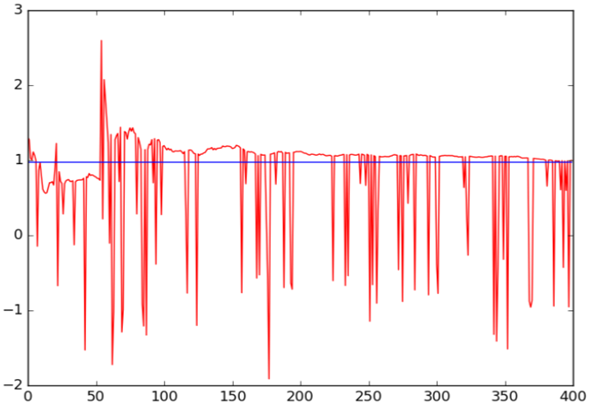
\includegraphics[scale=0.6]{AlgBandit}
	\caption[Resultado de la selección de brazo usando \textit{bandits}]{Resultado de la selección del mejor brazo usando la teoría de los \textit{bandits}}
	\label{AlgBandit}
\end{figure}

La oscilación de la línea roja se produce por la exploración que el algoritmo hace de otras alternativas diferentes a la que en cada momento parece ser la mejor. Tampoco dan los mismos valores aunque esté probando el mismo brazo, porque estos valores están siendo generado con una distribución normal, con media en el valor real (que también fue aleatorio), dentro de una desviación estándar que en este caso fue de 1. 

\subsection{Generador de la matriz de adyacencia}

Posteriormente se implementó el código que genera las matrices de adyacencia del grafo por etapas. Estas matrices debían ser escalonadas, debían obedecer a los requisitos de precedencia de nodos entre etapas y debía tener al menos un 1 en cada fila para garantizar la conexión de las etapas. Este código también se probó varias veces y siempre arrojó resultados adecuados. Un ejemplo de este resultado se muestra en la figura \ref{MatrizAy}.

\begin{figure} [H]
    \label{Resul2}
	\centering
	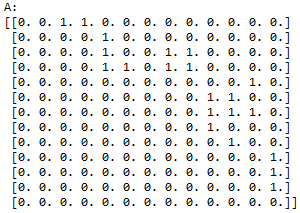
\includegraphics[scale=0.8]{MatrizAy}
	\caption{Resultado de la matriz de adyacencia para un grafo por etapas}
	\label{MatrizAy}
\end{figure}

\subsubsection{Generación de una ruta aleatoria}

Se implementó la fusión del algoritmo para la generación de la matriz de adyacencia, con el que genera los valores asociados a cada nodo o \textit{bandit}; el pseudocódigo correspondiente se probó con valores aleatorios, obteniendo siempre la matriz escalonada que se esperaba y los valores asociados a los \textit{bandits}.

Se le adicionó una funcionalidad para que tomara una ruta factible, teniendo en cuenta la matriz de adyacencia para encontrar los vecinos de cada nodo. La pruebas que se hicieron funcionaron siempre correctamente. Se procedió a probar que sobre esta ruta, calculara correctamente tanto la ganancia real asociada (teniendo en cuenta el vector de valores generados para los \textit{bandits}), como la ganancia distorsionada asociada a esa misma ruta (teniendo en cuenta el nuevo vector de valores distorsionados de los \textit{bandits}, el cual se genera con números aleatorios que siguen una distribución normal con media en el elemento del primer vector, dentro de una desviación estándar de 1). Las pruebas para esta implementación siempre funcionaron correctamente.

\subsection{Encontrando la ruta óptima}

\textit{Aquí se presentan dos momentos diferentes: Inicialmente aquel donde la escogencia del siguiente nodo de un camino, solo tiene que estar dentro del conjunto de vecinos del nodo actual, pero todos con la misma probabilidad de ser seleccionados; a este modelo le reconoceremos como Probabilidades Uniformes. Seguidamente se implementa la generación de la matriz de probabilidades de transición de pasar de un nodo a otro, la cual se basa en un fundamento matemático específico que se presentó en la sección \ref{mat} y del que se espera que converja a una única respuesta con la mejor ruta encontrada; a este le reconoceremos como Probabilidad Modelada.}

\subsection{Búsqueda con probabilidad uniforme}

Inicialmente los nodos de una etapa que sean adyacentes al nodo que ha sido seleccionado en la etapa anterior, tienen una probabilidad uniforme de que sean seleccionados. Este algoritmo se construye básicamente, incluyendo un contador de iteraciones para que el algoritmo de generación de rutas factibles se ejecute una cantidad dada de veces determinada y una selección de la ruta que al final de las iteraciones hubiera obtenido la ganancia promedio, para entregarla como respuesta. 

El pseudocódigo queda como se ve en el cuadro del algoritmo \ref{PsUniforme}, que con los datos de entrada y los generados aleatoriamente para el grafo, calcula una ruta de nodos de cada etapa, solamente teniendo en cuenta que el siguiente nodo forme parte de los vecinos del presente.

\begin{algorithm} [h]
\caption{L-n-bandit-Uniforme(L=Cantidad de etapas, M[L]=Nodos por etapa,
n=Cantidad de nodos)} \label{PsUniforme}
\begin{algorithmic}[1]
\STATE Generate: Ad[nxn] = Matriz de adyacencia
\STATE Generate: B[n] = Bandits reales
\FOR{t = 1 \TO T}
     \STATE Initialize: orig = 0
     \STATE Add: orig in path
     \FOR{l = 1 \TO L-1}
        \STATE Generate: $nvz_{orig}$ = vecinos de orig
        \STATE Random: ${dest \in nvz_{orig}}$
        \STATE $orig = dest$
        \STATE Add: orig in path
     \ENDFOR
     \STATE Calculate: $Gan_{path}$
\ENDFOR
\end{algorithmic}
\end{algorithm}

\subsection{Búsqueda con probabilidades aprendidas}
Posteriormente se implementó el cálculo de la matriz de probabilidades de transición con las fórmulas explicadas en la sección \ref{mat} cuyo pseudocódigo se muestra en el cuadro algorítmico \ref{Pseudo}. A diferencia del anterior, la selección del nodo siguiente al presente en cada ruta, no solo va a tener en cuenta la vecindad con este último, sino el valor que el nodo a seleccionar tenga asociado en la matriz de probabilidad de transición que aquí se genera y se actualiza, de acuerdo a las ganancias que reciba el camino, en cada iteración, como se explica en seguida.

\begin{algorithm}
\caption{L-n-bandit(L=Cantidad de etapas, M[L]=Nodos por etapa )
} 
\label{Pseudo}
\begin{algorithmic}[1]
\STATE Calculate: n=Cantidad de nodos
\STATE Initialize: v[n] = 0
\STATE Generate: Ad[nxn] = Matriz de adyacencia
\STATE Generate: B[n] = Bandits reales
\FOR{t = 1 \TO T}
     \STATE Initialize: orig = 0
     \STATE Add: orig in path
     \STATE $P(i \to j) = \frac{e^{v_j}}{\sum_k A_{i,k} e^{v_k}},$
     \STATE Generate: $Gan_{n}$
     \STATE $Gain_{path}$ = 0
     \FOR{l = 1 \TO L-1}
        \STATE Generate: $nvz_{orig}$ = vecinos de orig
        \STATE Select: $dest \in nvz_{orig}$  by $P(i \to j)$
        \STATE $orig = dest$
        \STATE Add: orig in path
        \STATE $Gain_{path}$ =+ $Gan_{orig}$
     \ENDFOR
     \IF{$Gain_{path} > 0$}
        \STATE v[n+1] = v[n] + $\delta$ by i $\in$ path
     \ELSE
        \STATE v[n+1] = v[n] - $\delta$ by i $\in$ path   
     \ENDIF    
\ENDFOR
\end{algorithmic}
\end{algorithm}

Para la primera iteración se maneja una probabilidad uniforme. Para las demás iteraciones, se calculan las probabilidades de transición entre nodos y en cada iteración selecciona un nodo de la etapa inicial, se calculan sus vecinos o nodos alcanzables y se selecciona el que mayor probabilidad de transición presente, para guardarlo en la ruta y proceder a hacer la búsqueda de sus vecinos en la siguiente etapa, hasta llegar a la última, usando siempre el mismo criterio de selección.

Una vez se conozca la ganancia o pérdida al final de la iteración, se actualizan los valores de preferencia de cada nodo de esa ruta, de acuerdo a la fórmula \ref{model3}, este valor se utiliza para calcular las nuevas probabilidades de transición con la fórmula \ref{model2}, que se tendrán en cuenta en la siguiente iteración. Cabe anotar que al final de cada etapa solo se afectan las probabilidades de transición de los nodos involucrados en la ruta seleccionada, pero que al iniciar cada iteración se cuenta con todas las modificaciones que hayan sufrido estas probabilidades en las iteraciones pasadas de la simulación.

La selección del siguiente vecino está fuertemente influenciada por las probabilidades de transición, constituyéndose en la explotación de los caminos preferidos, pero siempre deja un porcentaje de posibilidad de escoger cualquier nodo que no sea el de mayor probabilidad de transición asociada, lo que permite resolver el problema de la exploración, propio de la teoría de los \textit{bandits}, que garantiza la búsqueda de mejores soluciones que no se han considerado aún.

Al final de las iteraciones definidas, el simulador debe converger a la mejor ruta que haya estudiado, que puede ser la óptima, como se verá en la siguiente sección.

\section{Pruebas}

\subsection{Grafo para las pruebas}

Aunque el algoritmo se ha diseñado para generar grafos aleatorios, se hace necesario generar uno particular para poder comparar los valores resultantes de las ejecuciones del algoritmo con este. Tal grafo debe ser de un tamaño adecuado para poder calcular todas las posibles rutas desde un nodo inicial hasta uno final con sus respectivas ganancias; además, los nodos deberán tener asociados valores de ganancias, de forma que se pueda establecer claramente cuál es la ruta óptima.

Se decide entonces, trabajar con un grafo de 5 etapas y 13 nodos, dispuestos como se ve en la figura \ref{Grafomodelo}, pero no necesariamente con esas aristas, es decir, con matriz de adyacencia aleatoria, así como los valores de sus \textit{bandits}, pero obligando a que uno de ellos por etapa tuviese un mayor valor que los demás, para favorecer la ruta mejor y así verificar si estaba funcionando.

\begin{figure}[h]
  \centering
    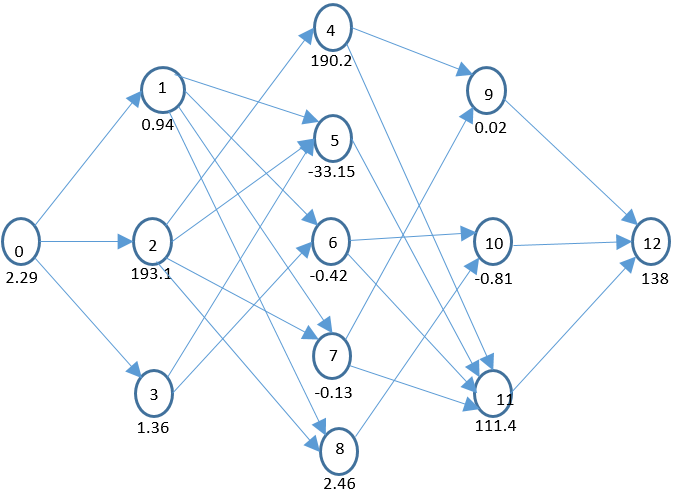
\includegraphics[scale=0.5]{Grafo5L.png}
  \caption[Grafo Modelo]{Grafo Modelo con 5 etapas y 13 nodos}
  \label{Grafomodelo}
\end{figure}


\subsection{Pruebas con probabilidad uniforme}

El algoritmo cuyo pseudocódigo se presentó en el cuadro \ref{PsUniforme}, se ejecutó con 99 intervalos de tiempo. La figura \ref{fig:uniforme} muestra uno de los resultados. 

\begin{figure}[H]
	\centering
	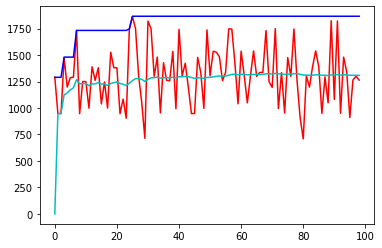
\includegraphics[scale=1]{Uniforme}
	\caption{Resultado con probabilidad uniforme}
	\label{fig:uniforme}
\end{figure}

En esta gráfica, la curva superior azul corresponde a la ganancia de la mejor ruta probada hasta el momento, calculada con el valor real de los \textit{bandits} o medias asignadas a cada uno; en la curva más inestable se presentan las ganancias obtenidas en cada instante de tiempo por la ruta seleccionada, calculada con los valores distorsionados de los \textit{bandits}, que fueron generados alrededor del vector B de las medias, con una desviación estándar de 1; y en la curva inferior verdosa se muestra el promedio acumulado de estas ganancias, el cual converge a un único valor a través del tiempo, pero no trata de acercarse al valor real.

\subsection{Pruebas con probabilidades aprendidas}

Con 33 iteraciones (T=33) el algoritmo \ref{Pseudo} generó la gráfica de la figura \ref{Resul2}, en la cual se pueden apreciar los valores que van tomado su ganancia y su ganancia promedio, la cual convergió rápidamente hacia el valor de la mejor ganancia real. La mejor ganancia real se calculó para la mejor ruta que el mismo algoritmo haya encontrado: esto permite que el software sea el que estime dicha ruta y su ganancia, sin una intervención manual, ya que hacer este cálculo equivaldría a una búsqueda exhaustiva en árbol, lo que puede llegar a ser muy dispendioso.

\begin{figure} [H]
	\centering
	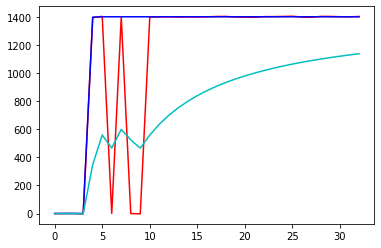
\includegraphics[scale=1]{Resul2}
	\caption{Resultado con probabilidad aprendida}
	\label{Resul2}
\end{figure}

En esta gráfica, al igual que en la del modelo anterior, la curva superior azul corresponde a la ganancia de la mejor ruta probada hasta el momento, calculada con el valor real de los \textit{bandits} o medias asignadas a cada uno; en la curva más inestable se presentan las ganancias obtenidas en cada instante de tiempo por la ruta seleccionada, calculada con los valores distorsionados de los \textit{bandits}, que fueron generados alrededor del vector B de las medias, con una desviación estándar de 1; y en la curva inferior verdosa se muestra el promedio acumulado de estas ganancias. 

De otra parte, era importante saber cómo se comportaba el algoritmo, al ejecutarlo varias veces, dejando fijos los datos de entrada correspondientes al grafo que se quería evaluar, por lo que de aquí en adelante no se generaron más matrices de adyacencia ni vectores reales de los \textit{bandits} aleatorios, sino que se dejaron valores fijos para ejecutar las pruebas que se explican en el siguiente capítulo.
